



\section*{Houdini section}
\markboth{\hspace{1cm}exercices}{Joris Putteneers\hspace{1cm}}



word\footnote{Explanation of the word.} that Addjword\footnote{Explanation of the word.} thatjord\footnote{Explanation of the word.} thatYou can find the source code on GitHub: \url{https://github.com/your-username/your-repository}.
%
%
%\begin*{figure}[H] 
%    \centering
%    \begin*{subfigure}[b]{0.49\textwidth}
%        \centering
%        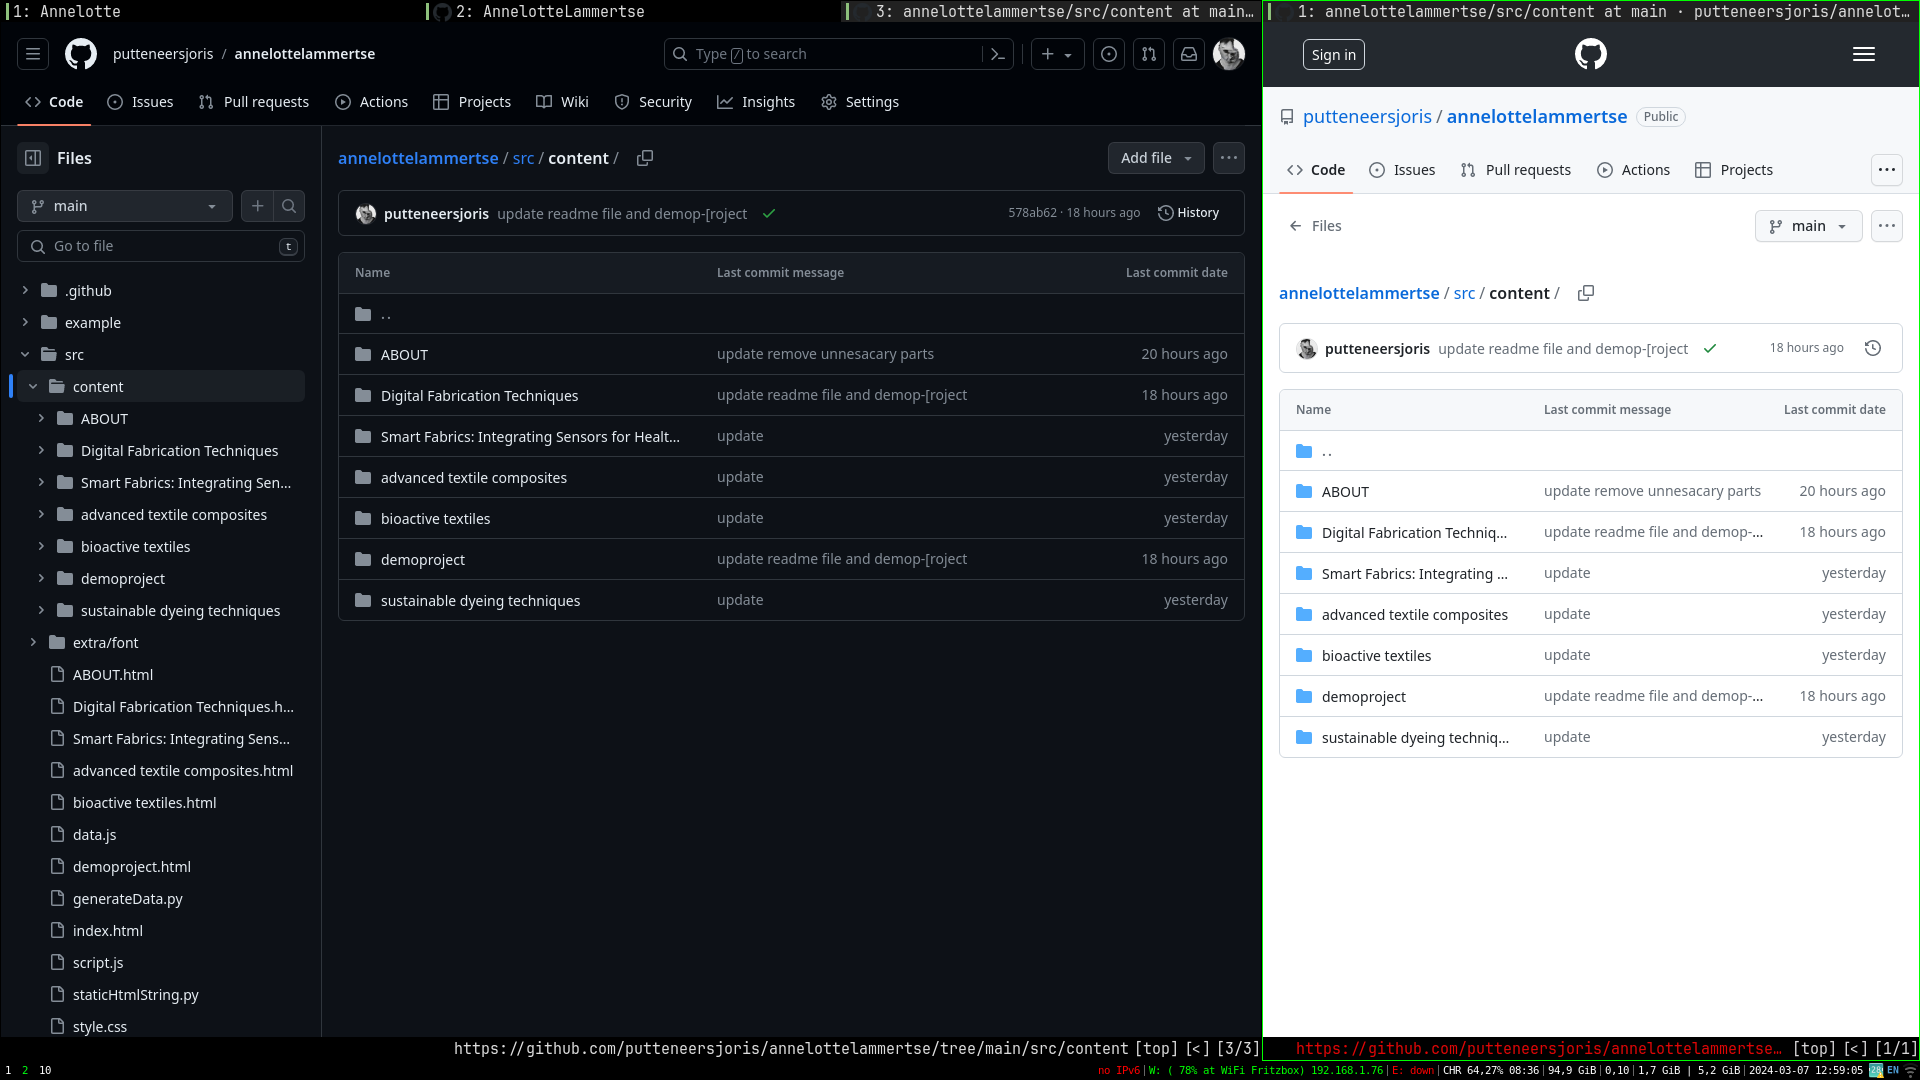
\includegraphics[width=1\textwidth]{sections/assignment_1/1.png}
%        \caption*{digital signal}
%    \end{subfigure}
%    \hfill
%    \begin*{subfigure}[b]{0.49\textwidth}
%        \centering
%        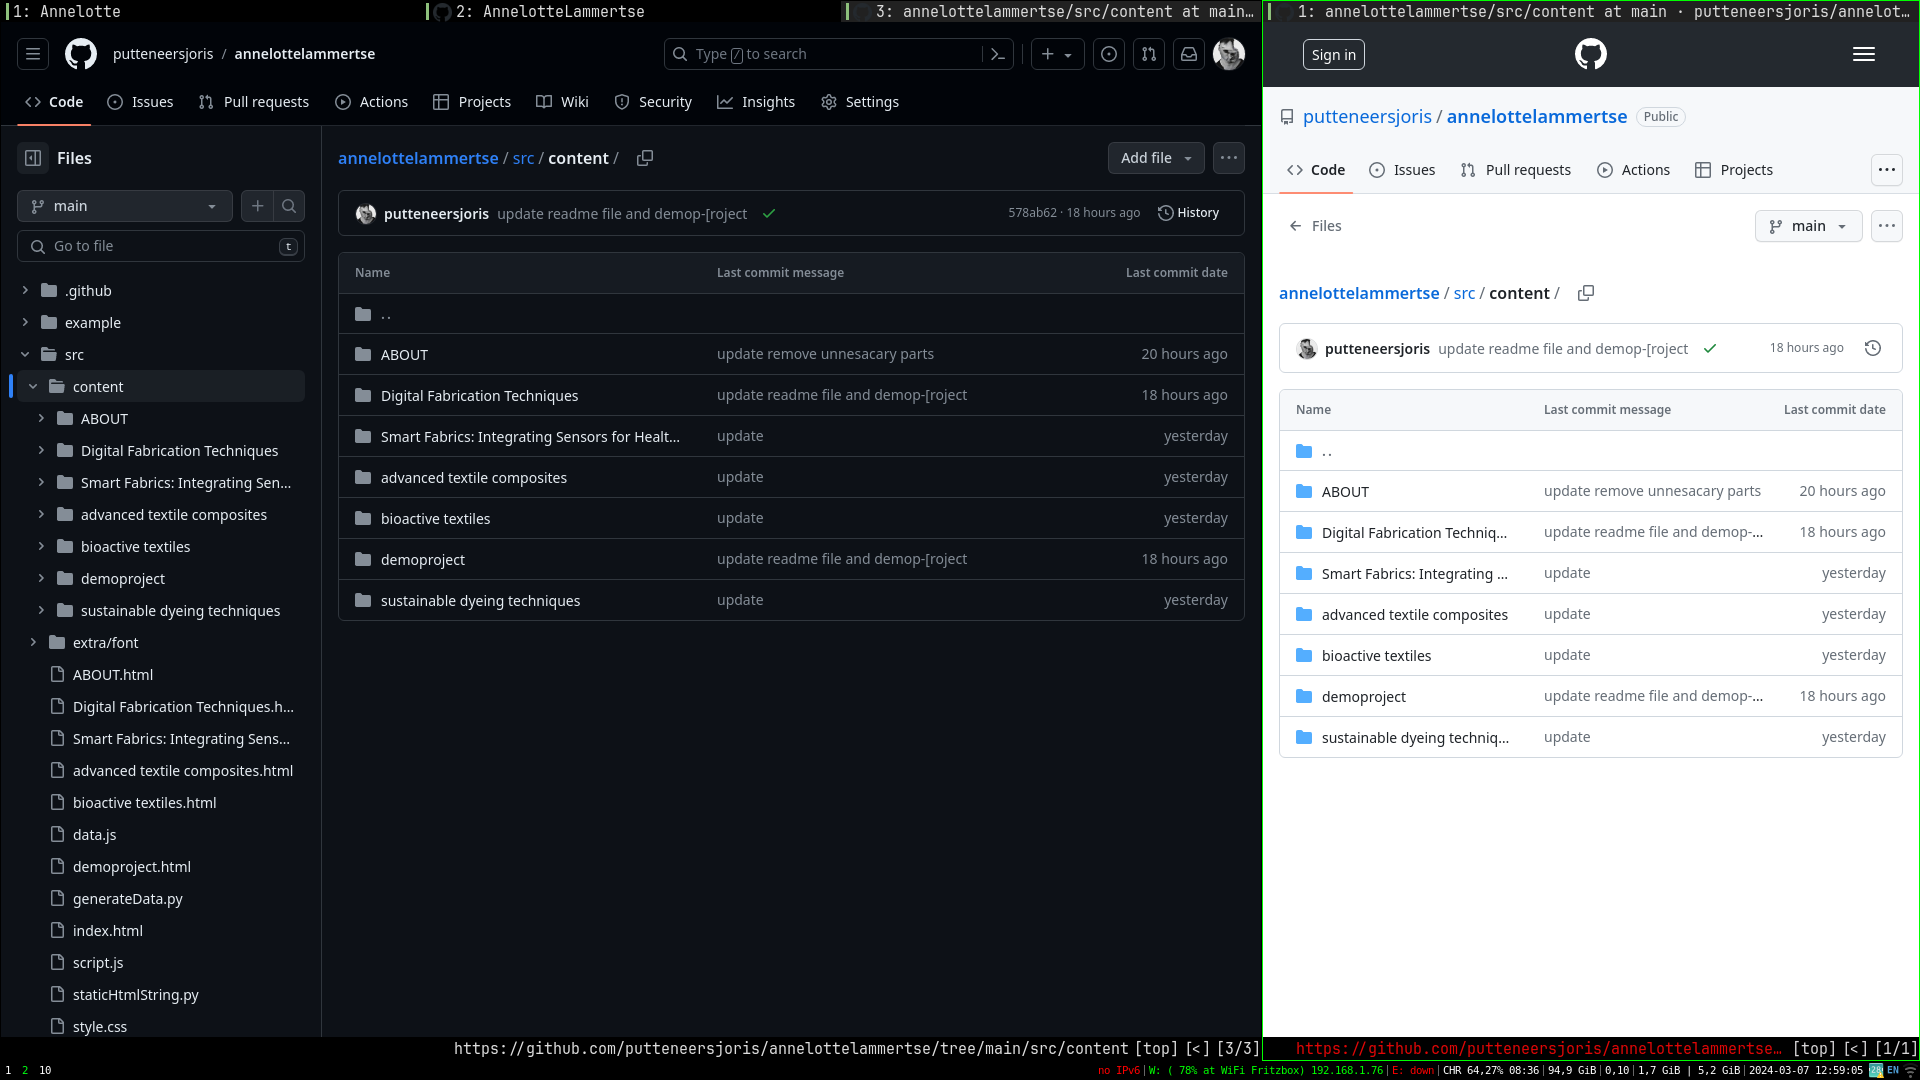
\includegraphics[width=1\textwidth]{sections/assignment_1/1.png}
%        \caption*{analog signali of the same signal that dispalyssi the same signal that dispalyssi the same signal that dispalyssi the same signal that dispalyssi the same signal that dispalyssi the same signal that dispalys} 
%    \end{subfigure}
%\end{figure}
%

\keywords{node / context / parameter / attribute / primitive /mitive mitive mitive mitive mitive  vertex / point / object / procedural / datatype}




A node is a fundamental building block in Houdini. It is a container that holds data and has a specific function. Nodes can be connected to each other to create a network that defines the behavior of a scene. There are different types of nodes in Houdini, such as geometry nodes, shader nodes, and compositing nodes.

A context is a specific environment in which nodes operate. Each context has its own set of rules and parameters that define how nodes behave. For example, the geometry context is used for creating and manipulating geometry, while the shader context is used for defining the appearance of objects.

\lipsum[1-20]
A parameter is a value that can be adjusted to change the behavior of a node. Parameters are used to control the properties of nodes, such as the color of a light or the size of a sphere. Parameters can be adjusted manually by the user or driven by expressions or other nodes.

